% !TEX root = task-3-9-3.tex
% Editable task bank. Append new BankTask blocks at the end of the document.
\documentclass[12pt,a4paper]{article}
\usepackage{physics-textbook}
\usepackage{graphicx,needspace}
\usetikzlibrary{decorations.pathmorphing}
\newif\ifShowSolutions
\ifdefined\TutorEdition
  \ShowSolutionstrue
\else
  \ShowSolutionsfalse % Change to \ShowSolutionstrue to display solutions.
\fi
\newcounter{banktask}
\newsavebox{\BankTaskBox}
\newcommand{\BankTaskContent}[3]{%
  \noindent\textbf{\thebanktask.}\quad #2\par
  \ifShowSolutions
    \Needspace{50mm}% Keep the solution heading with its opening text or diagram.
    #3\par
    \ifdefined\TutorEdition
      \ifcsname TutorSource#1\endcsname
        \nopagebreak\smallskip{\small\csname TutorSource#1\endcsname\par}%
      \fi
    \fi
  \fi
}
\newcommand{\BankTask}[3]{%
  \refstepcounter{banktask}\par\medskip
  \sbox{\BankTaskBox}{\begin{minipage}{\linewidth}%
    \BankTaskContent{#1}{#2}{#3}\end{minipage}}%
  \ifdim\dimexpr\ht\BankTaskBox+\dp\BankTaskBox\relax>\dimexpr\textheight-20mm\relax
    \Needspace{35mm}\BankTaskContent{#1}{#2}{#3}%
  \else
    \Needspace{\dimexpr\ht\BankTaskBox+\dp\BankTaskBox\relax}%
    \noindent\usebox{\BankTaskBox}\par
  \fi
  \medskip
}
\begin{document}
\BookSubsection{3.9.3}{Удельное сопротивление}


% Source sdamgia-7355: https://phys-ege.sdamgia.ru/problem?id=7355
\BankTask{sdamgia-7355}{
В школьной лаборатории есть два проводника круглого сечения. Удельное сопротивление первого проводника в $2$ раза больше удельного сопротивления второго проводника. Длина первого проводника в $2$ раза больше длины второго. При подключении этих проводников к одинаковым источникам постоянного напряжения за одинаковые интервалы времени во втором проводнике выделяется количество теплоты в $4$ раза большее, чем в первом. Каково отношение радиуса второго проводника к радиусу первого проводника? Источник тока считать идеальным.\par
}{
\smallskip\noindent\textbf{Решение}\par
Количество теплоты, выделяемое на проводнике, согласно закону Джоуля — Ленца: $Q= ( \frac{ U ^2 }{ R } ) \cdot t.$\par
Сопротивление проводника: $R= \frac{ \rho l}{ S } = \frac{ \rho l}{ \pi r ^2 } .$\par
Запишем соотношение: $\frac{ 1}{ 4 } = \frac{ Q_{1}}{ Q_{2} } = \frac{ R_{2}}{ R_{1} } = \frac{ \rho_{2} l_{2} r_{1} ^2 }{ r_{2} ^2 \rho_{1} l_{1} } = \frac{ 1}{ 2 \cdot 2 } \frac{ r_{1} ^2 }{ r_{2} ^2 } .$\par
Отсюда:$\frac{ r_{2}}{ r_{1} } =1.$\par
Ответ: $1$.\par
}

% Source sdamgia-10223: https://phys-ege.sdamgia.ru/problem?id=10223
\BankTask{sdamgia-10223}{
При подключении куска проволоки к полюсам батареи через нее течет ток силой $0{,}5 \,\text{А}$. Этот кусок проволоки сложили пополам, место сгиба разрезали. Затем разрезали каждый получившийся короткий провод на две равные части, зачистили концы и присоединили все эти части к полюсам батареи параллельно. Найдите силу тока, которая будет течь через батарею в этом случае. Внутреннее сопротивление батареи очень мало.\par
}{
\smallskip\noindent\textbf{Решение}\par
Сопротивление длинного однородного проводника обратно пропорционально площади его сечения: $R= \frac{ \rho l}{ S } .$ Всю проволоку сопротивлением $R$ разрезали на $4$ равные части сопротивлением $R/4$ каждая. Общее сопротивление такой цепи при параллельном соединении будет равно $R_{0}=R/16.$ Тогда по закону Ома в цепи будет течь ток, в $16$ раз больший первоначального $I=16I_{0}=8\,\text{А}.$\par
Ответ: $8$.\par
}

% Source sdamgia-24367: https://phys-ege.sdamgia.ru/problem?id=24367
\BankTask{sdamgia-24367}{
По проволочному резистору течет ток. Как изменятся при уменьшении длины проволоки в $4$ раза и увеличении силы тока вдвое тепловая мощность, выделяющаяся на резисторе, и его электрическое сопротивление?\par
$1$. Увеличится.\par
$2$. Уменьшится.\par
$3$. Не изменится.\par
\begin{center}\small\setlength{\tabcolsep}{3pt}\begin{tabular}{|p{0.45\linewidth}|p{0.45\linewidth}|}\hline
Тепловая мощность,
выделяющаяся на резисторе & Электрическое сопротивление
резистора\\\hline
 & \\\hline
\end{tabular}\end{center}\par
}{
\smallskip\noindent\textbf{Решение}\par
Сопротивление проводника зависит от его длины прямо пропорционально. Следовательно, при уменьшении длины в $4$ раза его сопротивление уменьшится в $4$ раза ($2$).\par
Тепловая мощность, выделяемая в проводнике, вычисляется по формуле $P=I^{2}R$. Сила тока увеличится в $2$ раза, а сопротивление уменьшится в $4$ раза, следовательно, тепловая мощность не изменится ($3$).\par
Ответ: $32$.\par
}

% Source sdamgia-45485: https://phys-ege.sdamgia.ru/problem?id=45485
\BankTask{sdamgia-45485}{
Отрезок провода с большим удельным сопротивлением подключён к клеммам источника постоянного напряжения. Отрезок провода заменили другим проводом такой же длины и из того же материала, но вдвое большего диаметра. Как изменились в результате такой замены сопротивление внешней цепи и сила тока во внешней цепи? Считать, что напряжение на внешней цепи остаётся неизменным.\par
$1$) увеличилась\par
$2$) уменьшилась\par
$3$) не изменилась\par
\begin{center}\small\setlength{\tabcolsep}{3pt}\begin{tabular}{|p{0.45\linewidth}|p{0.45\linewidth}|}\hline
Сопротивление & Сила тока\\\hline
 & \\\hline
\end{tabular}\end{center}\par
}{
\smallskip\noindent\textbf{Решение}\par
Электрическое сопротивление рассчитывается по формуле $R = \frac{ \rho l}{ S } .$ При увеличении диаметра провода площадь его сечения увеличивается, а сопротивление уменьшается ($2$).\par
Тогда сила тока в цепи увеличивается ($1$).\par
Ответ: $21$.\par
}

% Source sdamgia-11805: https://phys-ege.sdamgia.ru/problem?id=11805
\BankTask{sdamgia-11805}{
Для проведения лабораторной работы по обнаружению зависимости сопротивления проводника от его диаметра ученику выдали пять проводников, характеристики которых приведены в таблице. Какие два из предложенных ниже проводников необходимо взять ученику, чтобы провести данное исследование?\par
\begin{center}\small\setlength{\tabcolsep}{3pt}\begin{tabular}{|p{0.225\linewidth}|p{0.225\linewidth}|p{0.225\linewidth}|p{0.225\linewidth}|}\hline
№
проводника & Длина проводника & Диаметр проводника & Материал\\\hline
$1$ & $100 \,\text{см}$ & $1{,}0 \,\text{мм}$ & медь\\\hline
$2$ & $200 \,\text{см}$ & $0{,}5 \,\text{мм}$ & медь\\\hline
$3$ & $200 \,\text{см}$ & $1{,}0 \,\text{мм}$ & медь\\\hline
$4$ & $100 \,\text{см}$ & $0{,}5 \,\text{мм}$ & алюминий\\\hline
$5$ & $300 \,\text{см}$ & $1{,}0 \,\text{мм}$ & медь\\\hline
\end{tabular}\end{center}\par
}{
\smallskip\noindent\textbf{Решение}\par
Для определения зависимости сопротивления проводника от его диаметра необходимо выбрать проводники, у которых все остальные параметры (длина и материал) одинаковы. Это проводники с номерами $2$ и $3$.\par
Ответ: $23$.\par
}

% Source sdamgia-24955: https://phys-ege.sdamgia.ru/problem?id=24955
\BankTask{sdamgia-24955}{
На графике показана зависимость силы тока $I$, текущего в цилиндрическом медном проводнике с площадью поперечного сечения $3{,}4 \,\text{мм}^{2}$, от приложенного к его концам напряжения $U$. Удельное сопротивление меди $0{,}017 \,\text{Ом} \cdot \,\text{мм}^{2}/\,\text{м}$.\par
Чему равна длина этого проводника? (В метрах.)\par

\begin{center}\begin{tikzpicture}[book diagram,>=stealth]
\draw[task grid,xstep=1,ystep=.5](0,0)grid(3,3);\draw[task axis](0,0)--(3.4,0)node[right]{$U,\,\text{В}$};\draw[task axis](0,0)--(0,3.4)node[above]{$I,\,\text{А}$};\node[below left]at(0,0){$0$};\foreach\x/\s in{1/.5,2/1.0}{\node[below]at(\x,0){$\s$};}\foreach\y in{1,2}\node[left]at(0,\y){$\y$};\draw[task curve](.8,.8)--(2.75,2.75);
\end{tikzpicture}\end{center}
\par
}{
\smallskip\noindent\textbf{Решение}\par
Сопротивление проводника равно $R= \frac{ U}{ I } ,$ $R= \frac{ \rho l}{ S } .$ Следовательно:\par
\[l= \frac{ US}{ \rho I } = \frac{ 1 \cdot 3{,}4}{ 2 \cdot 0{,}017 } =100\,\text{м}.\]
Ответ: $100$.\par
}

% Source sdamgia-36761: https://phys-ege.sdamgia.ru/problem?id=36761
\BankTask{sdamgia-36761}{
Участок цепи состоит из двух последовательно соединенных цилиндрических проводников, сопротивление первого из которых равно $R$, а второго $2R$. Как изменится общее сопротивление этого участка цепи и тепловая мощность, выделяющаяся в первом проводнике, если удельное сопротивление и площадь поперечного сечения первого проводника увеличить вдвое, оставив без изменения его длину и напряжение на концах участка цепи? Сопротивление второго проводника не меняется.\par
$1$. Увеличится.\par
$2$. Уменьшится.\par
$3$. Не изменится.\par
\begin{center}\small\setlength{\tabcolsep}{3pt}\begin{tabular}{|p{0.45\linewidth}|p{0.45\linewidth}|}\hline
Общее сопротивление участка цепи & Тепловая мощность, выделяющаяся
в первом проводнике\\\hline
 & \\\hline
\end{tabular}\end{center}\par
}{
\smallskip\noindent\textbf{Решение}\par
А) При увеличении площади сечения и удельного сопротивления первого проводника в $2$ раза его сопротивление не изменится. Поскольку проводники соединены последовательно, то общее сопротивление участка цепи не изменится ($3$).\par
Б) Поскольку сопротивление первого проводника и напряжение не изменились, то выделяющаяся в нем тепловая мощность также не изменится ($3$).\par
Ответ: $33$.\par
}

% Source sdamgia-4206: https://phys-ege.sdamgia.ru/problem?id=4206
\BankTask{sdamgia-4206}{
Школьник изучал процесс протекания постоянного тока через проволоку постоянного поперечного сечения $2 \,\text{мм}^{2}$. Изменяя длину проволоки $L$, он измерял при помощи миллиомметра ее сопротивление $R$. Результаты его измерений приведены в таблице.\par
\begin{center}\small\setlength{\tabcolsep}{3pt}\begin{tabular}{|p{0.129\linewidth}|p{0.129\linewidth}|p{0.129\linewidth}|p{0.129\linewidth}|p{0.129\linewidth}|p{0.129\linewidth}|p{0.129\linewidth}|}\hline
$L$, см & $50$ & $70$ & $90$ & $110$ & $130$ & $150$\\\hline
$R$, мОм & $103$ & $140$ & $175$ & $228$ & $260$ & $298$\\\hline
\end{tabular}\end{center}\par
Пользуясь таблицей, определите удельное сопротивление металла, из которого была изготовлена проволока. (Ответ дать в омах квадратного миллиметра на метр, округлив до десятых.)\par
}{
\smallskip\noindent\textbf{Решение}\par
Сопротивление проводника длиной $L$ с площадью поперечного сечения $S$ и с удельным сопротивлением $\rho$ равно $R= \frac{ \rho L}{ S } .$ Для каждого измерения сосчитаем удельное сопротивление $\rho = \frac{ RS}{ L }$\par
\begin{center}\small\setlength{\tabcolsep}{3pt}\begin{tabular}{|p{0.129\linewidth}|p{0.129\linewidth}|p{0.129\linewidth}|p{0.129\linewidth}|p{0.129\linewidth}|p{0.129\linewidth}|p{0.129\linewidth}|}\hline
$L$, см & $50$ & $70$ & $90$ & $110$ & $130$ & $150$\\\hline
$R$, мОм & $103$ & $140$ & $175$ & $228$ & $260$ & $298$\\\hline
$\rho,\,\text{Ом} \cdot \,\text{мм} ^2 /\,\text{м}$ & $0{,}41$ & $0{,}40$ & $0{,}39$ & $0{,}41$ & $0{,}40$ & $0{,}40$\\\hline
\end{tabular}\end{center}\par
Усредним полученные выражения:\par
\[\frac{ 0{,}41 + 0{,}40 + 0{,}39 + 0{,}41 + 0{,}40 + 0{,}40}{ 6 } \approx 0{,}4\,\text{Ом} \cdot \,\text{мм} ^2 /\,\text{м}.\]
Ответ: $0{,}4$.\par
}

% Source sdamgia-38950: https://phys-ege.sdamgia.ru/problem?id=38950
\BankTask{sdamgia-38950}{
Нихромовый проводник длиной $l=l_{2}$ включён в цепь постоянного тока. К нему подключают вольтметр таким образом, что одна из клемм вольтметра всё время подключена к началу проводника, а вторая может перемещаться вдоль проводника. На рисунке приведена зависимость показаний вольтметра $U$ от расстояния $x$ до начала проводника. Как зависит от $x$ площадь поперечного сечения проводника? Ответ поясните, указав, какие физические закономерности вы использовали.\par

\begin{center}\begin{tikzpicture}[book diagram,>=stealth]
\draw[task axis](0,0)--(3.7,0)node[right]{$x$};\draw[task axis](0,0)--(0,3.1)node[above]{$U$};\node[below left]at(0,0){$0$};\draw[task projection](1,0)--(1,1.7)--(0,1.7);\draw[task projection](3,0)--(3,2.7)--(0,2.7);\node[below]at(1,0){$l_1$};\node[below]at(3,0){$l_2$};\node[left]at(0,1.7){$U_1$};\node[left]at(0,2.7){$U_2$};\draw[task curve](0,0)--(1,1.7)--(3,2.7);
\end{tikzpicture}\end{center}
\par
}{
\smallskip\noindent\textbf{Решение}\par
Так как проводник включен в цепь постоянного тока, то выполняется закон Ома для участка цепи $I= \frac{ U}{ R } ,$ где сила тока $I$ одинакова на всех участках цепи, напряжение на обоих участках растет, судя по графику, линейно. Сопротивление проводника равно $R= \frac{ \rho x}{ S } ,$ где $S$ — площадь поперечного сечения. В силу линейной зависимости напряжения от длины на каждом участке делаем вывод, что площадь поперечного сечения при $0 < x < l_{1}$ постоянно и равно $S_{1},$ при $l_{1} < x < l_{2}$ также постоянно и равно $S_{2}.$\par
Учитывая, что на первом участке напряжение растет быстрее, чем на втором, делаем вывод, что площадь поперечного сечения второго участка больше, чем у первого $S_{2} > S_{1}.$\par
Ответ: площадь поперечного сечения постоянна на каждом участке и $S_{2} > S_{1}.$\par
}

% Source sdamgia-41152: https://phys-ege.sdamgia.ru/problem?id=41152
\BankTask{sdamgia-41152}{
По цилиндрическому проводнику с площадью поперечного сечения $S=2 \,\text{мм}^{2}$ протекает электрический ток силой $I=1 \,\text{А}$. Параллельно проводнику подключён плоский конденсатор. Модуль напряжённости электрического поля между пластинами этого конденсатора равен $E=50 \,\text{В/м}$. Найдите удельное электрическое сопротивление $\rho$ данного проводника, если известно, что его длина в $n=1000$ раз больше расстояния между пластинами конденсатора.\par
}{
\smallskip\noindent\textbf{Решение}\par
$1$. По закону Ома для участка цепи напряжение между концами цилиндрического проводника равно $U_{R} = IR,$ где сопротивление проводника $R = \rho \frac{ l}{ S }$ ($l$ — длина проводника, $S$ — площадь его поперечного сечения).\par
$2$. Напряжение между пластинами плоского конденсатора $U_{C} = Ed,$ где $d$ — расстояние между пластинами.\par
$3$. Поскольку проводник и конденсатор соединены параллельно, $U_{C} = U_{R}.$ С учётом выражения для $R$ получим: $Ed = \frac{ I \rho l}{ S } .$ Отсюда\par
\[\rho = \frac{ ES}{ I } \cdot \frac{ d}{ l } = \frac{ ES}{ nI } = \frac{ 50\,\text{В/м} \cdot 2 \cdot 10 ^{ - 6 } \,\text{м} ^2 }{ 1000 \cdot 1\,\text{А} } = 0{,}1 \frac{ \,\text{Ом} \cdot \,\text{мм} ^2 }{ \,\text{м} } .\]
Ответ: $\rho = \frac{ ES}{ nI } = 0{,}1 \frac{ \,\text{Ом} \cdot \,\text{мм} ^2 }{ \,\text{м} } .$\par
}


% Source 328FBF: https://ege.fipi.ru/bank/questions.php?search=1&proj=BA1F39653304A5B041B656915DC36B38&qid=328FBF
\BankTask{328FBF}{
Для лабораторной работы по обнаружению зависимости сопротивления проводника от его длины ученику выдали пять проводников, характеристики которых указаны в таблице. Какие два из предложенных ниже проводников необходимо взять ученику, чтобы провести данное исследование?

\begin{center}
\begin{tabular}{|c|c|c|c|}
\hline
№ проводника & \shortstack{Длина проводника,\\\(\text{см}\)} & \shortstack{Диаметр проводника,\\\(\text{мм}\)} & Материал \\
\hline
\(1\) & \(200\) & \(1{,}0\) & алюминий \\
\hline
\(2\) & \(100\) & \(0{,}5\) & медь \\
\hline
\(3\) & \(100\) & \(1{,}0\) & медь \\
\hline
\(4\) & \(100\) & \(0{,}5\) & алюминий \\
\hline
\(5\) & \(200\) & \(1{,}0\) & медь \\
\hline
\end{tabular}
\end{center}
}{
\smallskip\noindent\textbf{Решение от GPT}\par
Сопротивление проводника \(R=\rho l/S\), поэтому при изменении длины нужно сохранить одинаковыми материал и диаметр проводников. Проводники \(3\) и \(5\) изготовлены из меди, имеют диаметр \(1{,}0\,\text{мм}\) и разные длины: \(100\,\text{см}\) и \(200\,\text{см}\). Ответ: \(35\).
}

% Source 837BC0: https://ege.fipi.ru/bank/questions.php?search=1&proj=BA1F39653304A5B041B656915DC36B38&qid=837BC0
\BankTask{837BC0}{
Для проведения лабораторной работы по обнаружению зависимости сопротивления проводника от его диаметра ученику выдали пять проводников, характеристики которых приведены в таблице. Какие два из предложенных ниже проводников необходимо взять ученику, чтобы провести данное исследование?

\begin{center}
\begin{tabular}{|c|c|c|c|}
\hline
№ проводника & Длина проводника & Диаметр проводника & Материал \\
\hline
\(1\) & \(100\,\text{см}\) & \(1{,}0\,\text{мм}\) & медь \\
\hline
\(2\) & \(200\,\text{см}\) & \(0{,}5\,\text{мм}\) & медь \\
\hline
\(3\) & \(200\,\text{см}\) & \(1{,}0\,\text{мм}\) & медь \\
\hline
\(4\) & \(100\,\text{см}\) & \(0{,}5\,\text{мм}\) & алюминий \\
\hline
\(5\) & \(300\,\text{см}\) & \(1{,}0\,\text{мм}\) & медь \\
\hline
\end{tabular}
\end{center}
}{
\smallskip\noindent\textbf{Решение от GPT}\par
Сопротивление проводника \(R=\dfrac{4\rho l}{\pi d^2}\), поэтому для исследования зависимости от диаметра нужно выбрать проводники одинаковых длины и материала. Проводники \(2\) и \(3\) изготовлены из меди и имеют длину \(200\,\text{см}\), а их диаметры различны: \(0{,}5\,\text{мм}\) и \(1{,}0\,\text{мм}\). Ответ: \(23\).
}

% Source 20041: https://phys-ege.sdamgia.ru/problem?id=20041
\BankTask{20041}{
\begin{center}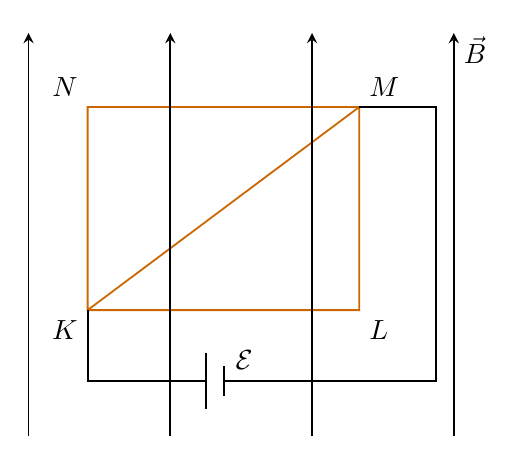
\begin{tikzpicture}[>=stealth,line width=.65pt]\draw[orange!80!black](.75,.9)rectangle(4.2,3.48) (.75,.9)--(4.2,3.48);\draw(.75,.9)--(.75,0)--(2.25,0) (2.48,0)--(5.17,0)--(5.17,3.48)--(4.2,3.48);\draw(2.25,-.35)--(2.25,.35) (2.48,-.19)--(2.48,.19);\node[above right]at(2.5,.02){$\mathcal E$};\foreach \x in {0,1.8,3.6,5.4}{\draw[->](\x,-.7)--(\x,4.42);} \node[below left]at(.75,.9){$K$};\node[above left]at(.75,3.48){$N$};\node[above right]at(4.2,3.48){$M$};\node[below right]at(4.2,.9){$L$};\node[right]at(5.4,4.2){$\vec B$};\end{tikzpicture}\end{center}

Из медной проволоки с удельным сопротивлением $\rho$  =  $1{,}7$ · $10^{-8}$ Ом · м и площадью поперечного сечения S  =  $0{,}2\,\text{мм}^{2}$ изготовлен прямоугольный контур KLMN с диагональю KM (см. рис.). Стороны прямоугольника KL  =  $l_{1}$  =  $20\,\text{см}$ и LM  =  $l_{2}$  =  $15\,\text{см}$. Контур подключили за диагональ к источнику постоянного напряжения с ЭДС $\mathcal{E}$  =  $1{,}4\,\text{В}$ и поместили в однородное магнитное поле с индукцией В  =  $0{,}1$ Тл, параллельной сторонам KN и LM. С какой результирующей силой магнитное поле действует на контур? Сделайте рисунок с указанием сил, действующих на контур. Внутренним сопротивлением источника пренебречь.
}{
\smallskip\noindent\textbf{Решение}\par
\begin{center}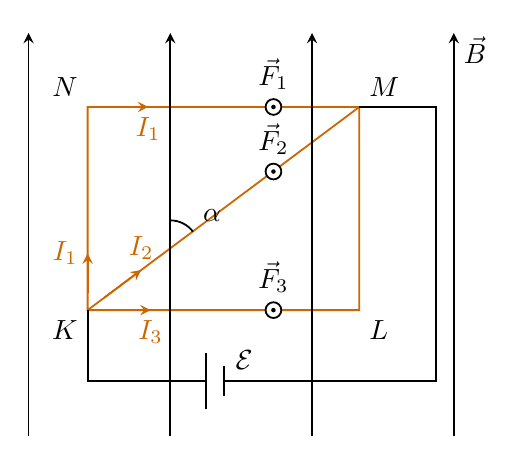
\begin{tikzpicture}[>=stealth,line width=.65pt]\draw[orange!80!black](.75,.9)rectangle(4.2,3.48) (.75,.9)--(4.2,3.48);\draw(.75,.9)--(.75,0)--(2.25,0) (2.48,0)--(5.17,0)--(5.17,3.48)--(4.2,3.48);\draw(2.25,-.35)--(2.25,.35) (2.48,-.19)--(2.48,.19);\node[above right]at(2.5,.02){$\mathcal E$};\foreach \x in {0,1.8,3.6,5.4}{\draw[->](\x,-.7)--(\x,4.42);}\draw[->,orange!80!black](.75,1.12)--(.75,1.62)node[left]{$I_1$};\draw[->,orange!80!black](1,3.48)--(1.52,3.48)node[below]{$I_1$};\draw[->,orange!80!black](.96,1.057)--(1.43,1.409)node[above]{$I_2$};\draw[->,orange!80!black](.99,.9)--(1.55,.9)node[below]{$I_3$};\foreach \x/\y/\i in {3.11/3.48/1,3.11/2.66/2,3.11/.9/3}{\draw[fill=white](\x,\y)circle(.1);\fill(\x,\y)circle(.029);\node[above]at(\x,\y+.09){$\vec F_{\i}$};}\draw(1.8,2.04)arc(90:37:.36)node[above right]{$\alpha$};\node[below left]at(.75,.9){$K$};\node[above left]at(.75,3.48){$N$};\node[above right]at(4.2,3.48){$M$};\node[below right]at(4.2,.9){$L$};\node[right]at(5.4,4.2){$\vec B$};\end{tikzpicture}\end{center}

$1$.  При подключении контура к источнику напряжения по его сторонам и диагонали потекут токи $I_{1}$, $I_{2}$ и $I_{3}$ (см. рис.). Проводники KNM, KLM и KM соединены параллельно, следовательно, $I_1=I_3= \frac{\mathcal{E}}{R_1}$ и $I_2= \frac{\mathcal{E}}{R_2} ,$ где $R_1=\rho \cdot \frac{l_1 + l_2}{S}$ и $R_2=\rho \cdot \frac{l}{S}$ $( KM=l= \sqrt{l_1 ^2 + l_2 ^2} )$  — сопротивления соответствующих проводников.
$2$.  Со стороны магнитного поля на проводники KL и NM, перпендикулярные индукции магнитного поля, а также на диагональ KM действуют силы Ампера: $F_1=F_3=BI_1l_1,$ и $F_2=BI_2l \sin \alpha ,$ где $\sin \alpha = \frac{l_1}{l} .$ По правилу левой руки силы Ампера параллельны друг другу и направлены к наблюдателю, на проводники KN и ML сила Ампера не действует. Таким образом, результирующая сила $F = 2F_1 + F_2.$
$3$.  Выполняя преобразования, получим:

$F_1= \frac{B\mathcal{E} Sl_1}{\rho ( l_1 + l_2 )}$ и $F_2= \frac{B\mathcal{E} Sl_1}{\rho \sqrt{l_1 ^2 + l_2 ^2}} .$

В итоге:

$F=2F_1 + F_2=2 \frac{B\mathcal{E} Sl_1}{\rho ( l_1 + l_2 )} + \frac{B\mathcal{E} Sl_1}{\rho \sqrt{l_1 ^2 + l_2 ^2}} = \frac{B\mathcal{E} Sl_1}{\rho} ( \frac{2}{l_1 + l_2} + \frac{1}{\sqrt{l_1 ^2 + l_2 ^2}} ) =$

$= \frac{0{,}1 \cdot 1{,}4 \cdot 0{,}2 \cdot 10 ^{ - 6 } \cdot 0{,}2}{1{,}7 \cdot 10 ^{ - 8 }} ( \frac{2}{0{,}2 + 0{,}15} + \frac{1}{\sqrt{0{,}2 ^2 + 0{,}15 ^2}} ) =3{,}2 \,\text{Н}.$

Ответ: F  =  $3{,}2$ Н.
}

\end{document}
